%% FEUP THESIS STYLE for LaTeX2e
%% how to use feupteses (portuguese version)
%%
%% FEUP, JCL & JCF, 31 Jul 2012
%%
%% PLEASE send improvements to jlopes at fe.up.pt and to jcf at fe.up.pt
%%

%%========================================
%% Commands: pdflatex tese
%%           bibtex tese
%%           makeindex tese (only if creating an index) 
%%           pdflatex tese
%% Alternative:
%%          latexmk -pdf tese.tex
%%========================================

\documentclass[11pt,a4paper,twoside,openright]{report}

%% For iso-8859-1 (latin1), comment next line and uncomment the second line
\usepackage[utf8]{inputenc}
%\usepackage[latin1]{inputenc}

%% Portuguese version

%% MIEEC options
\usepackage[portugues,mieec]{feupteses}
%\usepackage[portugues,mieec,juri]{feupteses}
%\usepackage[portugues,mieec,final]{feupteses}
%\usepackage[portugues,mieec,final,onpaper]{feupteses}

%% For other degrees
% \usepackage[portugues]{feupteses} % you must define the degree below

%% Options: 
%% - portugues: titles, etc in portuguese
%% - onpaper: links are not shown (for paper versions)
%% - backrefs: include back references from bibliography to citation place

%% Uncomment to create an index (at the end of the document)
%\makeindex

%% Path to the figures directory
%% TIP: use folder ``figures'' to keep all your figures
\graphicspath{{figures/}}

%%----------------------------------------
%% TIP: if you want to define more macros, use an external file to keep them
%some macro definitions

% format
\newcommand{\class}[1]{{\normalfont\slshape #1\/}}

% entities
\newcommand{\Feup}{Faculdade de Engenharia da Universidade do Porto}

\newcommand{\svg}{\class{SVG}}
\newcommand{\scada}{\class{SCADA}}
\newcommand{\scadadms}{\class{SCADA/DMS}}

%%----------------------------------------

%%========================================
%% Start of document
%%========================================
\begin{document}

%%----------------------------------------
%% Information about the work
%%----------------------------------------
\title{Implementação em FPGA de um conversor HDMI para transmissão ótica em série}
\author{Ana Marisa Oliveira Barbosa}


%% Uncomment next line for date of submission
%\thesisdate{31 de Julho de 2008}

%% Comment next line for copyright text if not used
\copyrightnotice{Marisa Oliveira, 2017}

\supervisor{Orientador}{Prof. Doutor João Paulo de Castro Canas Ferreira}
\supervisor{Co-orientador}{Prof. Dr. Henrique Manuel de Castro Faria Salgado}
\supervisor{Supervisor Externo}{Dr. Luís Manuel de Sousa Pessoa}

%% Uncomment next line if necessary
%\supervisor{Co-orientador}{Nome de Outro Orientador}

%% Uncomment committee stuff in the final version if used
%\committeetext{Aprovado em provas públicas pelo Júri:}
%\committeemember{Presidente}{Nome do presidente do júri}
%\committeemember{Arguente}{Nome do arguente do júri}
%\committeemember{Vogal}{Nome do vogal do júri}
%\signature

%% Specify cover logo (in folder ``figures'')
\logo{uporto-feup.pdf}
 
%% Uncomment next line for additional text  below the author's name (front page)

%%----------------------------------------
%% Preliminary materials
%%----------------------------------------

% remove unnecessary \include{} commands
\begin{Prolog}
  \chapter*{Resumo}
%\addcontentsline{toc}{chapter}{Resumo}

A sociedade atual depende cada vez mais dos serviços de comunicações, exigindo melhores ligações e mais rápidas, prevendo-se num futuro próximo a necessidade de ligações na ordem das centenas de \SI{}{\giga\bit\per\second}. O projeto \textit{iBrow} que está a ser desenvolvido por vários parceiros, incluindo o INES-TEC, vem propor uma nova exploração do espetro de frequências permitindo assim comunicações de alta velocidade. Este projeto passa por propor uma metodologia que permite a manufaturação de transcetores de baixo custo capazes de atingir grandes débitos de transmissão. A interface HDMI é cada vez mais usada em todos os tipos de ambientes: tanto empresariais como domésticos. Por esse motivo acaba por ser uma boa interface para testar os transcetores que estão a ser desenvolvidos. E por isso, nesta dissertação, é proposto um projeto cuja motivação passa por testar os mesmos. 

O trabalho realizado consiste no desenvolvimento e implementação de  uma arquitetura em FPGA capaz de suportar sinais provenientes de uma fonte HDMI, serializá-los e ainda enviá-los a alta velocidade. A arquitetura suporta ainda o processo inverso, isto é, recebe os dados em série em alta velocidade e envia-os de seguida para um dispositivo HDMI de destino. Para cumprir os requisitos propostos o projeto é dividido em duas partes.

Numa primeira fase são desenvolvidas arquiteturas que permitem a comunicação entre dois dispositivos recorrendo a duas placas HDMI e uma FPGA \textit{Xilinx 	Virtex} 7 para realizar tal transmissão. Estas variam entre a transmissão de imagem em diferentes formatos e também de imagem e som. Numa segunda fase do projeto desenvolve-se uma arquitetura capaz de serializar dados e enviá-los pelas saídas de alta velocidade disponíveis na FPGA utilizada. Esses mesmo dados são recebidos de volta na FPGA e convertidos para o seu formato original. Por fim, englobando as duas partes, conseguiu-se obter a transmissão em série de dados HDMI.

\chapter*{Abstract}
%\addcontentsline{toc}{chapter}{Abstract}


Our society is increasingly dependent on communication services, demaning better and faster connections, reaching in a near future the order of hundreds of \SI{}{\giga\bit\per\second}. The \textit{iBrow} project, which is being developed by several partners, including INESC-TEC, comes with a new proposal of the frequency spectrum exploitation, allowing high-speed communications. This project also proposes a methodology that allows the manufacturing of low budget transceivers capable of reaching big transmission rates. The HDMI interface is increasingly used in all kinds of environment: from enterprises until domestic use. For that reason it is a good interface to test the transceivers that are being developed. Therefore, in this dissertation is proposed a project whose motivation is to test the \textit{iBrow} transceivers.

The progress work is based on the development and implementation of a design on the FPGA that is able to support signals from an HDMI sink, serialized them and send it through a high-speed channel. This architecture allows the reverse process, in other words, it is able to receive the high-speed serial data and send it to and HDMI source. To accomplish the proposed goals, the project is divided in two parts.

The firts step proposes architectures that allow the communication between two devices using two HDMI boards and a Xilinx Virtex 7 FPGA to reach the transmission. These architectures differs from each other regarding the kind of the transmission: different formats of image, or support of image and sound.

In the second phase of the project, an architecture which is able to serialize data and send it through the FPGA high-speed outputs is developed. It also supports the reception of the serial data and do the reverse process, which is convert it to its original format.

Finally, one can reach the final result by joining the two phases of the project, which is obtain a serial communication between HDMI sink and source.


 % the abstract
  \chapter*{Agradecimentos}
%\addcontentsline{toc}{chapter}{Agradecimentos}

Agradecer a toda a gente no mundo.
\vspace{10mm}
\flushleft{O Nome do Autor}
  % the acknowledgments
  \cleardoublepage
\thispagestyle{plain}

\vspace*{8cm}

\begin{flushright}
   \textsl{``Nada se perde, nada se cria, tudo se transforma''} \\
\vspace*{1.5cm}
           Antoine Lavoisier
\end{flushright}
    % initial quotation if desired
  \cleardoublepage
  \pdfbookmark[0]{Conteúdo}{contents}
  \tableofcontents
  \cleardoublepage
  \pdfbookmark[0]{Lista de Figuras}{figures}
  \listoffigures
  \cleardoublepage
  \pdfbookmark[0]{Lista de Tabelas}{tables}
  \listoftables
  \chapter*{Abreviaturas}
%\addcontentsline{toc}{chapter}{Abbreviations}
\chaptermark{ABREVIATURAS E SÍMBOLOS}

\begin{flushleft}
\begin{tabular}{l p{0.8\linewidth}}
ARC			& 	\textit{Audio Return Channel} 																			\\
BER			&	\textit{Bit Error Rate}																					\\
CDR			&	\textit{Clock Data Recovery}																			\\
CEC			& 	\textit{Consumer Electronics Control}																	\\
CMU			& 	\textit{Clock Multiplier Unit}																			\\
DDC			&	\textit{Display Data Channel}																			\\
DFE			&	\textit{Decision Feedback Equalizer}																	\\
DVI			&	\textit{Digital Video Interface}																		\\
EDID		&	\textit{Extended Display Identification Channel}														\\
EEPROM		&	\textit{Electrically erasable programmable read-only memory}											\\
EIA/CEA 	&	\textit{Electronic Industry Alliance/ Consumer Eletronics Association}									\\
FEC			&	\textit{Forward Error Correction}																		\\
FEUP      	& 	Faculdade de Engenharia da Universidade do Porto 														\\
FIFO		&	\textit{First-In First-Out}																				\\
FMC			&	\textit{FPGA Mezzanine Cards}																			\\
FPGA		&	\textit{Field-Programmable Gate Array}																	\\
HDCP		&	\textit{High-bandwith Digital Content Protection}														\\
HDMI		&	\textit{High Definition Multimedia Interface}															\\
HDTV		&	\textit{High-Definition television}																		\\
HEC 		&	\textit{HDMI Ethernet Channel}																			\\
HPC			&	\textit{High Pin Count}																					\\
iBrow 		&	\textit{Innovative ultra-BROadband ubiquitous Wireless communications through terahertz transceivers}	\\
INESC-TEC	&	Instituto de Nacional de Engenharia de Sistema e Computadores Tecnologias e Ciências					\\
LPCM 		&	\textit{Linear Pulse Code Modulation}																	\\
MIMO		&	\textit{Multiple Input Multiple Output}																	\\
PCS			&	\textit{Physical Coding Sublayer}																		\\	
PISO		&	\textit{Parallel-Input Serial-Output}																	\\
PLL			&	\textit{Phase-Locked Loop}																				\\
PMA			&	\textit{Physical Medium Attachment Sublayer}															\\
PRBS		&	\textit{Pseudo Random Bit Sequence}																		\\
QAM			&	\textit{Quadrature Amplitude Modulation}																\\
RTD			&	\textit{Resonant Tunneling Diode}																		\\
SIPO		&	\textit{Serial-Input Parallel-Output}																	\\
TMDS		&	\textit{Transition- Minimized Differential Signaling}													\\
VESA		&	\textit{Video Electronics Standards Association}														\\
RGB			&	\textit{Red Green Blue}																									\\
I2S				&	\textit{Inter-IC Sound	}																											
\end{tabular}
\end{flushleft}

  % the list of abbreviations used
\end{Prolog}

%%----------------------------------------
%% Body
%%----------------------------------------

\StartBody

%% TIP: use a separate file for each chapter
\chapter{Introdução} \label{chap:intro}

Este trabalho surge no contexto do desenvolvimento do projeto realizado no âmbito na Unidade Curricular Dissertação, pertencente ao plano de estudos do Mestrado Integrado em Engenharia Eletrotécnica de Computadores. Nesta secção é feita uma análise introdutória do projeto, quer do ponto de vista geral em que este se enquadra, quer do ponto de vista motivacional do mesmo. Por fim, é feita uma descrição do problema dos objetivos do mesmo e da estrutura desta dissertação. 


\section{Enquadramento Geral} \label{sec:context}
Ao longo das últimas décadas a sociedade tem vindo a tornar-se cada vez mais dependente das comunicações com e sem fios, não só em termos empresariais, mas também pessoais. Esta tendência tem vindo a vincar-se recentemente com a crescente utilização de \textit{tablets} e \textit{smartphones}, tornando os recursos atuais incapazes de responder a tal procura. E cada vez mais esta exigência irá aumentar prevendo-se a necessidade de ligações na ordem das dezenas de \SI{}{\giga\bit\per\second} no ano de 2020, essencialmente para comunicações a curta distância sem fios segundo  segundo \cite{R040}. Daqui conclui-se que os recursos que existem atualmente não são capazes de responder a esta necessidade crescente de comunicações de alto débito, e como tal é necessário urgentemente o desenvolvimento de tecnologias não só capazes de satisfazer esta procura, mas ao mesmo tempo que o façam de forma eficiente em termos energéticos e financeiros. Neste contexto enquadra-se o projeto \textit{iBrow} (\textit{Innovative ultra-BROadband ubiquitous Wireless communications through terahertz transceivers}), o qual está a ser parcialmente desenvolvido pela equipa de investigação de tecnologias óticas e eletrónicas do INESC-TEC (Instituto de Nacional de Engenharia de Sistema e Computadores Tecnologias e Ciências), que vem responder a esta necessidade de uma forma eficiente.

O projeto \textit{iBrow} vem propor o desenvolvimento de uma tecnologia capaz de responder a esta necessidade de comunicações de alto débito através de uma utilização eficaz do espetro de frequências promovendo a utilização de bandas de frequência mais altas, desde \SI{60}{\giga\hertz}  até \SI{1}{\tera\hertz}. Para além disso vem também propor uma metodologia, que pela primeira vez permite um baixo custo de manufaturação de transcetores capazes de atingir altos débitos de transmissão para que possam ser perfeitamente integrados em redes de comunicações ótica de grande velocidade.
 
Todo este crescente de consumo por parte dos utilizadores de novas e cada vez mais tecnologias não se verifica apenas na necessidade de aumento de largura de banda para as comunicações, mas existe também uma necessidade extrema da existência de interfaces digitais de vídeo e som que não só sejam capazes de fazer chegar ao utilizador sinais de alto débito, mas que ao mesmo tempo o façam de maneira segura no sentido de proteger eventuais cópias não autorizadas. Assim sendo, o desenvolvimento de um conversor HDMI \textit{(High Definition Multimedia Interface}) de alto débito enquadra-se perfeitamente nesta necessidade sendo que é a interface de vídeo e áudio \textit{standard} e que implementa o protocolo HDCP (\textit{High-bandwith Digital Content Protection}) que protege a reprodução de sinais em dispositivos não autorizados.

Existem várias interfaces digitais que implementam o protocolo referido anteriormente, entre elas destacam-se \textit{DisplayPort}, DVI (\textit{Digital Visual Interface}) e HDMI. No entanto, devido ao tremendo sucesso que a interface HDMI obteve, de acordo com \textit{In-Stat} referido em \cite{R002} foram vendidos 5 milhões de exemplares em 2004, 17,4 milhões em 2005, 63 milhões em 2006 e 143 milhões em 2007, tornou-se a interface \textit{standard} para HDTV (\textit{High-Definition Television}), substituindo a interface DVI. Relativamente à interface \textit{DisplayPort}, esta é utilizada em vários equipamentos, mas principalmente no setor dos computadores e vem complementar o HDMI. Contudo, comparando as duas interfaces previamente referidas, o HDMI tem algumas vantagens no que toca à capacidade de transmitir sinais CEC (\textit{Consumer Electronics Control}) e a compatibilidade elétrica com o DVI. Mas o que destaca esta interface é a sua capacidade de transmissão dos sinais na sua largura de banda completa até 10 metros, enquanto que a \textit{DisplayPort} apenas o consegue transmitir até 3 metros.

Através da implementação dos objetivos propostos pela dissertação será possível implementar um conversor HDMI capaz de fazer transmitir sinais de alto débito, tornando mais eficiente este tipo de comunicações e ao mesmo tempo fazendo-o de forma segura, protegendo as cópias e reproduções não autorizadas dos sinais transmitidos.
 

\section{Motivação} \label{sec:goals}
Com a explosão que se fez sentir nos últimos anos na utilização do espetro de frequências, verifica-se que é necessário tornar a sua utilização mais eficiente no sentido de conseguir satisfazer a necessidade da sociedade de comunicar quase sem limites em termos de velocidade da comunicação em si. Promove-se assim uma nova abordagem do espetro de frequências, de maneira a que se possa utilizá-lo de uma forma mais eficaz.  
Ao longos dos anos tem-se vindo a verificar melhorias no que toca à eficiência espetral através do desenvolvimento e aplicação de algumas técnicas, tal como referido em \cite{R007}, como por exemplo o QAM (\textit{Quadrature Amplitude Modulation}) para modulação do sinal e também técnicas MIMO (\textit{Multiple Input Multiple Output}) nas entradas e saídas do sistema de comunicação. Verificou-se que o aproveitamento do espetro de facto melhorou, no entanto, estas técnicas não são suficientes para se conseguir atingir um débito de algumas dezenas ou centenas de \SI{}{\giga\bit\per\second}. Assim sendo, a solução passa por promover a utilização de bandas de frequência mais altas, contrariamente ao que se fez no passado.  

Por definição, considera-se a banda de ondas mm entre 60 a \SI{100}{\giga\hertz} e a banda THz entre \SI{100}{\giga\hertz} a \SI{1}{\tera\hertz}. Estas bandas do espetro de frequências são bandas cuja utilização no passado foi pouca ou até mesmo nenhuma, isto porque para conseguir explorar estas bandas são necessários componentes adequados à operação nas mesmas. Relativamente à banda de ondas mm, apesar de nos últimos anos terem sidos desenvolvidas e aplicadas técnicas que melhoram a eficiência espetral desta região, tal como referido anteriormente, a escassez da largura de banda limita o débito da ligação. Em \cite{R007} são referidas implementações realizadas no passado que conseguiram alcançar débitos até  \SI{100}{\giga\bit\per\second} em ligações sem fios a uma distância de 1 metro com BER (\textit{Bit Error Ratio}) igual a \num{1e-3} recorrendo também à utilização de mais de um transmissor e recetor. Apesar de inovadores estes valores revelam-se insuficientes para o que se pretende alcançar. 

Quanto à região do espetro que corresponde a uma frequência superior a \SI{10}{\tera\hertz}, apesar da grande largura de banda disponível nesta região, existem várias limitações para a comunicação sem fios referidas em \cite{R005}. Destaca-se o facto do baixo balanço de potência possível para a transmissão devido aos limites de segurança dos olhos, os impactos atmosféricos na propagação do sinal (chuva, pó e poluição) e ainda o impacto da falta de alinhamento entre transmissores e recetores. Estas são algumas das razões que limitam a comunicação sem fios para frequências superiores a \SI{10}{\tera\hertz}.

Assim sendo, segundo \cite{R005}, torna-se evidente que a banda do espetro com maior potencial para a comunicação sem fios é a banda entre \SI{100}{\giga\hertz} e \SI{1}{\tera\hertz}, uma vez que não só oferece uma largura de banda bastante maior (desde \SI{}{\giga\hertz} até \SI{1}{\tera\hertz}) comparativamente a outra bandas, mas também é uma região do espetro que não sofre muito devido às más condições atmosféricas. Para além disso, a utilização destas bandas de frequência altas acabará por aliviar o espetro relativamente à sua escassez e às suas limitações de capacidade. 

Tendo em conta esta nova abordagem do espetro, o projeto iBrow tem vindo a desenvolver metodologias que permitem a manufaturação de transcetores para operar a estas frequências de baixo custo, mas que ao mesmo tempo são capazes de atingir altos débitos, para que desta maneira sejam integrados em redes de comunicação com e sem fios de grande velocidade. Os transcetores de baixo custo propostos pelo projeto passam por utilizar díodos ressonantes de efeito túnel (RTD - \textit{Resonant Tunneling Diode}) com formatos de modulação simples e com interligação com fibra ótica. Assim, será possível satisfazer as necessidades previstas para 2020 de forma eficaz tanto em termos energéticos como financeiros.


A principal motivação do projeto proposto nesta dissertação passa por desenvolver um trabalho que possa demonstrar o potencial da tecnologia proposta pelo \textit{iBrow}, recorrendo à transmissão de vídeo em alta definição descomprimido pelos dispositivos propostos pelo projeto. Para efetuar a transmissão é utilizada a interface HDMI, que faz transmitir um sinal de alto débito para de seguida o mesmo sinal ser transmitido pelos transcetores propostos pelo projeto iBrow. Esta transmissão terá de ser realizada em série visto que estes mesmos transcetores apenas suportam transmissão de dados em série.

O HDMI é uma interface digital que transmite vídeo não comprimido e áudio que poderá ou não estar comprimido. Esta interface implementa vários protocolos entre quais se destaca o protocolo HDCP pois é o responsável pela prevenção de reproduções não autorizadas dos sinais a transmitir, o que é bastante importante hoje em dia dado os inúmeros consumidores que conseguem fazer cópias ilegais. Este protocolo faz uma verificação inicial antes de transmitir os dados encriptados no sentido de perceber se o dispositivo de destino é efetivamente um dispositivo autorizado para a reprodução de sinal. Esta é ainda uma interface que consegue transmitir sinais de alta definição e é ainda compatível com o DVI. Hoje em dia, esta é a interface \textit{standard} para HDTVs e tem diversas aplicações tais como câmaras digitais, discos \textit{Blu-ray} e leitores de DVD (\textit{Digital Video Disc}) de alta definição, computadores pessoais, \textit{tablets} e \textit{smartphones}.

Em suma, esta implementação torna-se bastante útil, uma vez que é capaz de abranger um vasto nível de aplicações acessíveis a todos os utilizadores, tanto em ambientes empresariais como pessoais.

%\section{Objetivos} \label{sec:struct}
%Este trabalho tem como principal objetivo a implementação de uma arquitetura de serialização e deserialização de um sinal HDMI, e que ao mesmo tempo faça o tratamento destes mesmos sinais para posterior envio e receção do sinal de alta velocidade em série. Como tal, será necessário utilizar um recurso que permita a implementação dessa mesma arquitetura versatilmente, por outras palavras, um recurso que permita eventuais reconfigurações da arquitetura desenvolvida e que ao mesmo tempo possua características que sejam úteis ao desenvolvimento do projeto.
%
%O projeto fará uso então de uma FPGA VC7203 Virtex-7 que possibilita a implementação de uma arquitetura adequada e que ao mesmo tempo possui entradas e saídas de alta velocidade que vão ajudar na ligação do sinal com os transcetores de alta velocidade. O protótipo desenvolvido em hardware reprogramável deve ser devidamente validado para que o sinal digital possa de seguida ser transmitido através de uma ligação por fibra ótica usando os RTDs desenvolvidos no projeto iBrow.

\section{Descrição do Problema e Objetivos} \label{sec:descrição_objetivos}

Este projeto tem como principal objetivo a implementação de uma arquitetura que permita a receção de dados HDMI, o seu tratamento e serialização para o seu posterior envio em alta velocidade. Para além disto, a arquitetura deve também receber os dados em série, fazer a sua conversão para paralelo e voltar a enviar para um dispositivo HDMI final.

\begin{figure}[h!]
	\begin{center}
		\leavevmode
		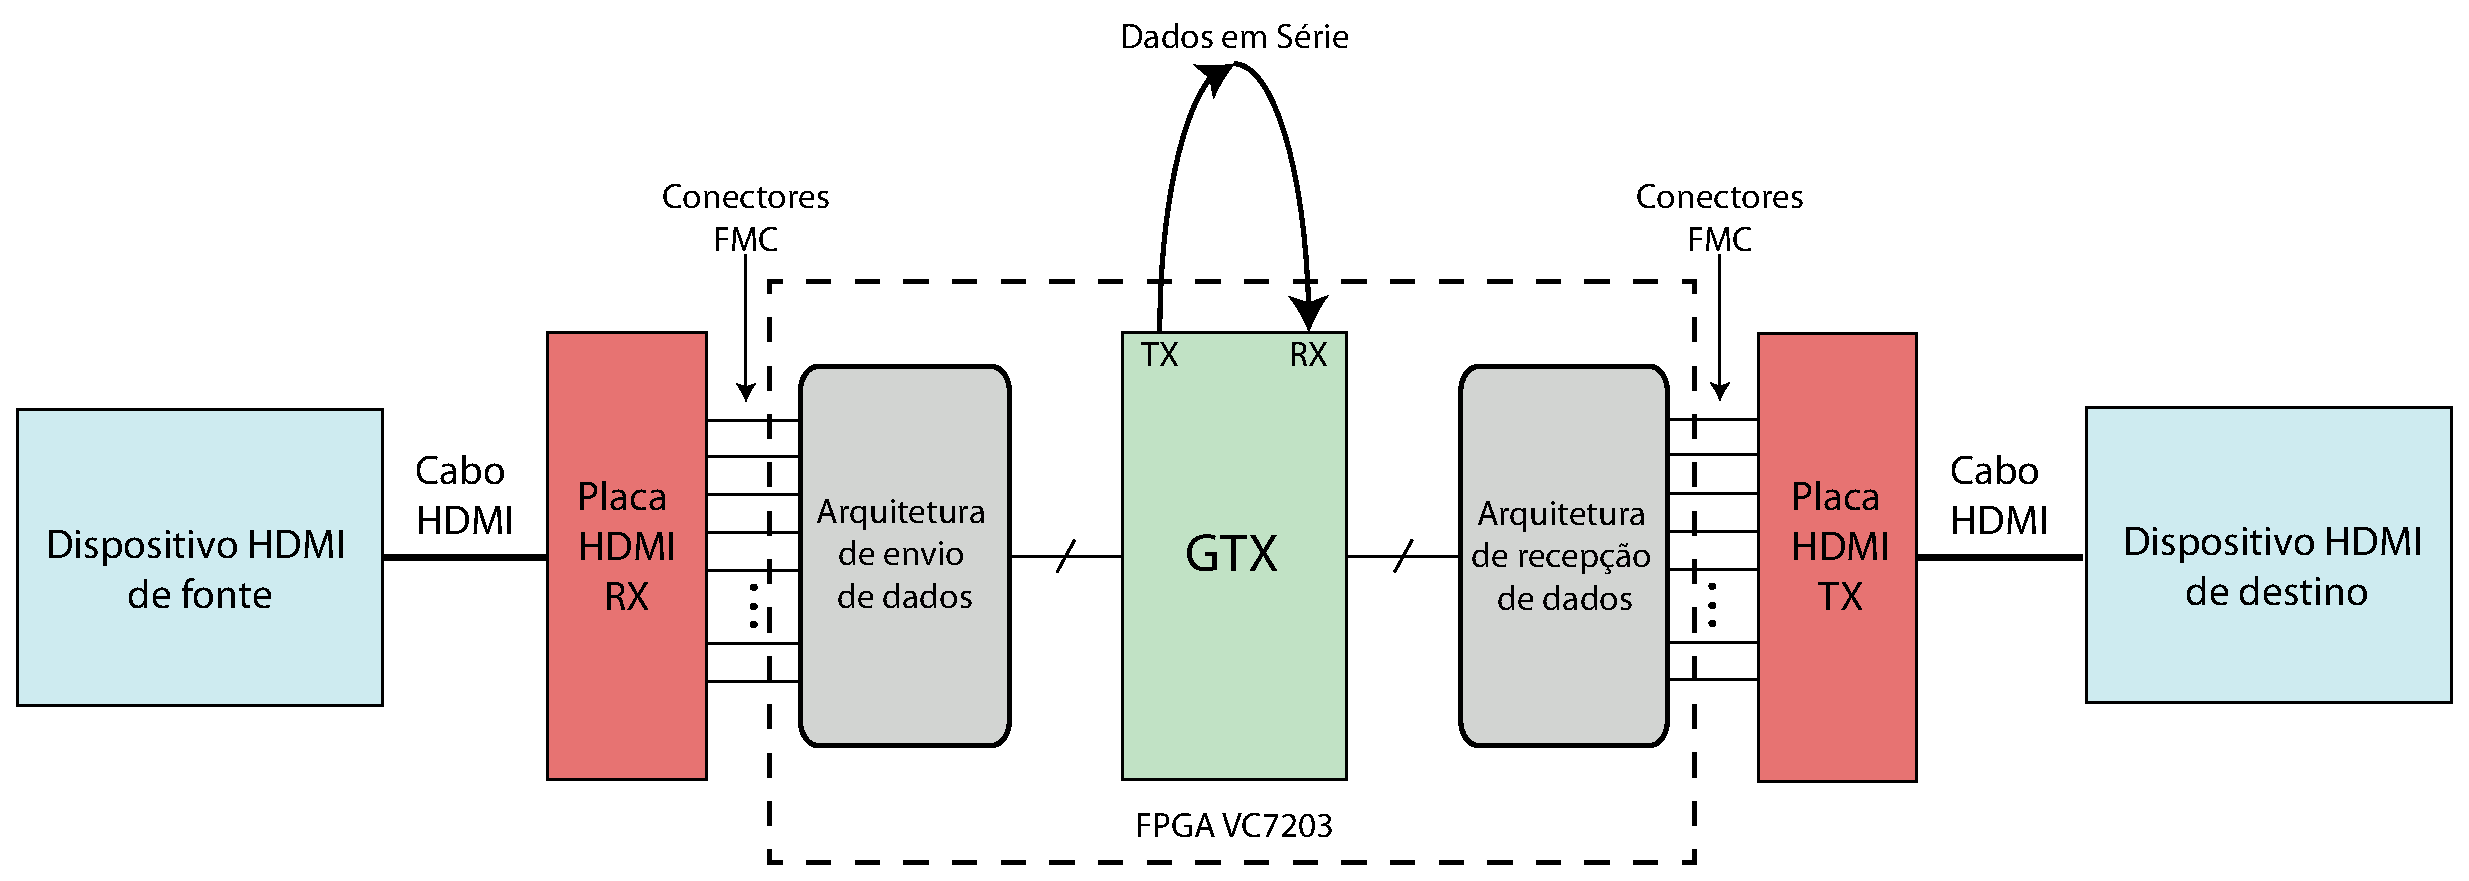
\includegraphics[width=1.0\textwidth]{diagrama_inicial}
		\caption{Diagrama geral do problema proposto}
		\label{fig:diagrama_inicial}
	\end{center}
\end{figure}

O projeto faz uso de uma FPGA (\textit{Field-Programmable Gate Array}) VC7203 (\textit{Virtex-7}) que possibilita a implementação de uma arquitetura adquada e ao mesmo tempo possui entradas e saídas de alta velocidade para testar a arquitetura desenvolvida. Para além disso, são também utilizadas umas placas HDMI que permitem enviar os dados em paralelo de um fonte HDMI para a FPGA VC7203 através dos conectores FMC (\textit{FPGA Mezzanine Cards}), e depois fazer o processo inverso, ou seja, enviar os dados em paralelo para a placa transmissora para que esta os transmita para o dispositivo final HDMI.

A figura \ref{fig:diagrama_inicial}  ilustra o diagrama geral do projeto a ser realizado. No sentido de simplificar o seu desenvolvimento, este foi dividido em duas partes:
\begin{enumerate}
	\item Conceção e desenvolvimento de arquiteturas que permitam comunicação entre dispositivos HDMI.
	\item Conceção e desenvolvimento de arquiteturas que permitem serialização de dados e deserialização dos mesmos.
\end{enumerate}

A primeira parte do projeto consiste em obter comunicações entre dois dispositivos HDMI utilizando para tal as placas HDMI disponíveis. A figura \ref{fig:1parte_projeto} ilustra um diagrama que descreve a primeira parte do projeto.
\begin{figure}[h!]
	\begin{center}
		\leavevmode
		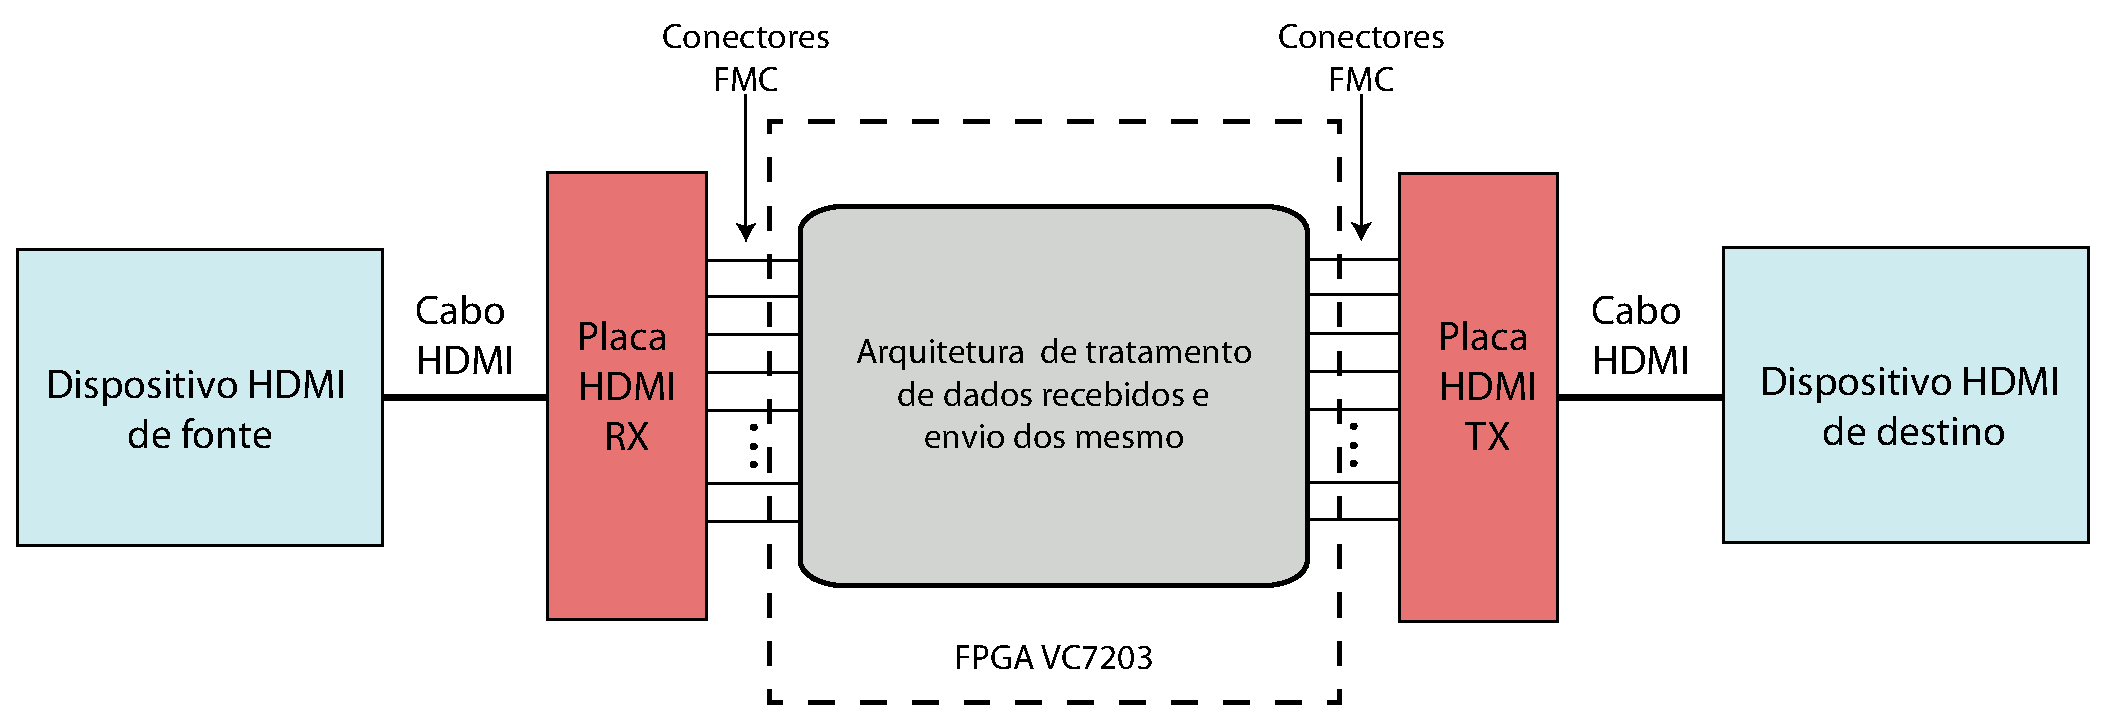
\includegraphics[width=1.0\textwidth]{1aparte}
		\caption{Diagrama geral da primeira parte do problema}
		\label{fig:1parte_projeto}
	\end{center}
\end{figure}

À placa HDMI recetora é ligado um sinal externo via cabo HDMI de uma fonte e de seguida essa mesma placa envia para a FPGA, através dos conectores FMC, os sinais de vídeo a serem transmitidos. Na FPGA VC7203 é desenvolvida uma arquitetura que permite o tratamento dos dados provenientes dos conectores FMC e de seguida, esses mesmo dados, são enviados para a placa HDMI transmissora de maneira a que esta os transmita para o dispositivo de destino.

A segunda parte do projeto consiste em desenvolver uma arquitetura na FPGA que permite serializar os dados recebidos enviá-los através das saídas de alta velocidade da mesma e voltar a recebê-los. A figura \ref{fig:2parte_projeto} ilustra o diagrama do trabalho a ser desenvolvido nesta fase.

\begin{figure}[h!]
	\begin{center}
		\leavevmode
		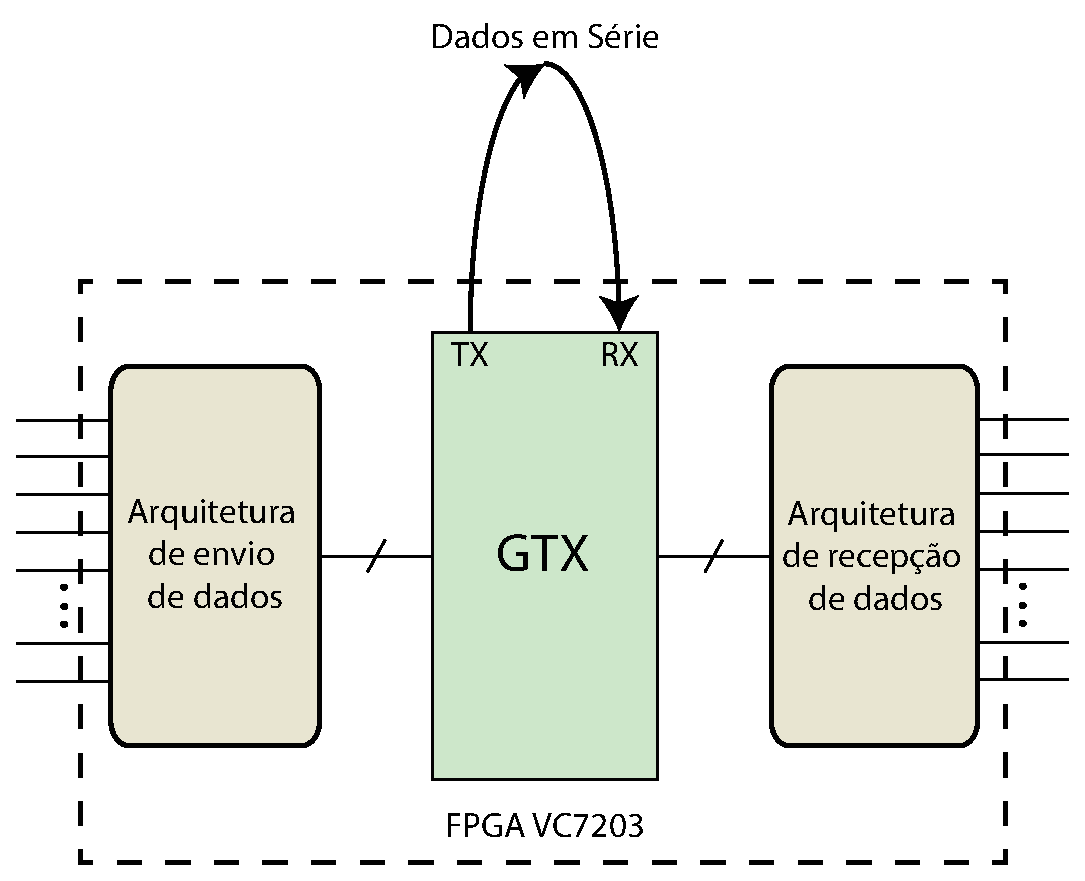
\includegraphics[width=0.7\textwidth]{2parte}
		\caption{Diagrama geral da segunda parte do problema}
		\label{fig:2parte_projeto}
	\end{center}
\end{figure}

Tal como ilustra a figura \ref{fig:2parte_projeto}, deve ser desenvolvida uma arquitetura que organize os dados em paralelo em tramas e de seguida os envie para os transcetores da FPGA que automaticamente fazem a sua serialização. Os dados em série são transmitidos por um cabo físico e recebidos nos transcetores onde são deserializados novamente. Por fim, as tramas são recebidas e processadas de modo a obter-se na saída os dados em paralelo tal como recebidos na entrada. Assim que as duas partes do projeto estejam concluídas obtém-se o objetivo final.

\section{Estrutura da Dissertação} \label{sec:struct}

Esta dissertação está organizada em vários capítulos que vão desde uma revisão bibliográfica do problema até à descrição da resposta ao mesmo. 
No capítulo \ref{chap:chap2} é feita uma revisão bibliográfica sobre os diversos aspetos que o problema apresenta, expondo também considerações de diversos autores sobre esses mesmos aspetos.  

No capítulo \ref{chap:chap3} é descrita toda a conceção e desenvolvimento das arquiteturas referentes à primeira parte do trabalho apresentado em \ref{sec:descrição_objetivos}. Todas estas são devidamente detalhadas e são ainda apresentados os principais resultados obtidos.

O capítulo \ref{chap:chap4} aborda todas as questões relativas à transmissão em série. Uma vez que existem transcetores disponíveis nos recursos utilizados, neste capítulo são apresentadas as arquiteturas dos mesmo e as características mais relevantes para o correto funcionamento do projeto em geral. No capítulo \ref{chap:chap5} são apresentas as arquiteturas desenvolvidas para se obter uma ligação em série, todas as suas características e ainda são explicadas as decisões tomadas quanto à escolha de determinados parâmetros.

O capítulo \ref{chap:concl} expõe as conclusões finais de todo o trabalho realizado e ainda aborda trabalho que pode futuramento ser realizado decorrente do que foi realizado até ao momento.

 
\chapter{Revisão Bibliográfica} \label{chap:sota}

Neste capítulo é realizada uma revisão bibliográfica das interfaces áudio e vídeo existentes, em específico do HDMI, também sobre métodos de codificação/descodificação de sinais HDMI numa FPGA e ainda sobre ligações de alta velocidade em série e cuidados que se deve ter com as mesmas.

\section{Interfaces de transmissão de video/audio}

As interfaces de áudio e vídeo definem parâmetros físicos e interpretações dos sinais recebidos, segundo \cite{R004}. Para sinais digitais a interface acaba por definir não só a camada física mas também a camada de ligação de dados e principalmente a camada da aplicação. As características físicas do equipamento (elétrico ou ótico) incluem o número e o tipo de ligações necessárias, tensões, frequências, intensidade ótica e ainda o design físico dos conectores. Relativamente à camada de ligação de dados, esta define como os dados da aplicação serão encapsulados para que, por exemplo, possam ser sincronizados ou para fazer correções de erros. Por fim, a camada da aplicação define o formato do sinal de áudio e vídeo a ser transmitido, normalmente incorporando \textit{codecs} não específicos. No entanto, por vezes esta camada acaba por não definir em concreto o tipo de formato de dados deixando em aberto tal parâmetro para que se possa transmitir dados no geral (é o caso do HDMI). No caso dos sinais analógicos, todas as funções que existem para os sinais digitais definidas em três camadas, são representadas num único sinal.

No caso da transmissão de sinais de áudio e vídeo digital existem várias interfaces que passam a ser analisadas, segundo \cite{R004}:
\begin{itemize}
	\item \textbf{\textit{Display Port:}} utiliza um conector do tipo \textit{DisplayPort} e é o principal concorrente do HDMI. Esta interface define uma interconexão sem licenças que foi inicialmente desenhada para ser utilizada numa conexão entre o computador e o monitor do mesmo. O sinal de vídeo não é compatível com DVI ou HDMI, mas um conector \textit{DisplayPort} pode fazer passar estes sinais.
	\item \textbf{\textit{ IEEE 1394 “FireWire":}} utiliza um conector do tipo \textit{FireWire} ou i.LINK. Este protocolo de transferência de dados é principalmente utilizado em câmaras digitais, mas também em computadores e em transferências de sinal de áudio. Este tipo de interface é capaz de hospedar vários sinais no mesmo cabo entregando os dados nos devidos destinos.
	\item \textbf{\textit{HDMI (High Definition Multimedia Interface):}} utiliza um conector do tipo HDMI e é uma interface de transmissão de sinal áudio/vídeo comprimida para transmissão de sinal digital descomprimida. 
\end{itemize}

\section{HDMI (\textit{High Definition Multimedia Interface})}\label{sec:dialecto}
O HDMI é uma interface de áudio e vídeo de alta definição que transporta dados áudio no formato não comprimido. Suporta num único cabo qualquer formato de vídeo em diversas resoluções e desde 2004 tem vindo a sofrer algumas alterações que vêm melhorar o desempenho da interface. 

Esta interface está dividida em diversos canais de comunicação que implementam determinados protocolos, entre os quais se destacam as seguintes de \cite{R002}:
\subsection{DDC - \textit{Display Data Channel} } \label{batik} 
É um conjunto de protocolos utilizado nas comunicações digitais entre um dispositvo de origem e um dispositivo final que permite a comunicação entre ambos. Estes protocolos permitem que o ecrã comunique com o seu adaptador quais os modos que consegue suportar e também que o dispositivo que liga ao ecrã consiga ajustar alguns parâmetros, como por exemplo o contraste e a luminosidade. EDID (\textit{Extended display identification data}) é a estrutura \textit{standard} para este tipo de comunicações que define as capacidades do monitor e os modos gráficos suportados pelo mesmo.  Este protocolo é utilizado pela \textit{source} da comunicação do HDMI para obter os dados necessários do dispoistivo \textit{sink}, no sentido de perceber quais os modos suportados pelo mesmo. Este canal é também ativamente usado para HDCP (\textit{High-Bandwith Digital Content Protection}).

\subsection{TMDS - \textit{Transition-Minimized Differential Signaling} } \label{batik} 
É uma tecnologia utilizada para transmissão de dados em série de alta velocidade utilizado em comunicações digitais. O transmissor implementa um algoritmo que reduz as interferências eletromagnéticas nos cabos e permite ainda uma recuperação robusta de sinal de relógio no recetor. 

Em específico na interface HDMI, este protocolo divide a informação a transmitir em 3 principais pacotes e intercala a sua transmissão: Período de transmissão de vídeo, período de transmissão de dados e período de controlo. No primeiro período (período de transmissão de vídeo) são transmitidas os pixeis do vídeo em linha. No segundo período (o período de transmissão de dados) são transmitidos os dados de vídeo e os dados auxiliares à transmissão dentro dos respectivos pacotes. O terceiro período ocorre entre os dois anteriores. 

Para além de ser utilizada no HDMI, esta técnica é também utilizada em interfaces DVI.
\subsection{CEC - \textit{Consumer Electronics Control} } \label{batik} 
É uma característica do HDMI que permite ao utilizador controlar até 15 dispositivos que tenham esta mesma característica ativa e que estão conectados por HDMI usando apenas um controlo remoto. Também é possivel dispositivos inviduais controlarem outros dispositivos sem intervenção do utilizador

\subsection{ARC - \textit{Audio Return Channel}  } \label{batik} 
Esta característica do HDMI utiliza 2 pins do conector. É uma ligação de audio que tem como objetivo substituir outros cabos entre a TV e outros recetores ou então sistema de som. Esta direção é usada quando é a TV que gera ou recebe o vídeo mas é outro equipamente que reproduz o som. Esta característica está apenas disponível a partir da versão 1.4 de HDMI.

\subsection{HEC - \textit{HDMI Ethernet Channel}  } \label{batik} 
Esta especificação do HDMI, tal como a anterior, está também apenas disponível a partir da versão 1.4 do HDMI e é uma tecnologia capaz de consolidar vídeo, audio e dados em série num único cabo HDMI, permitindo também aplicações baseadas em IP sobre o HDMI e uma comunicação \textit{Ethernet} bidireccional até 100 Mbit/s.

Uma das principais características mais recentes das interfaces HDMI prende-se ao facto de permitir que sinais não sejam reproduzidos em dipositivos não autrizados. Isto é, através de um protocolo cujo nome já foi referido anteriormente, HDCP (\textit{High-Bandwith Digital Content Protection}), o sinal HDMI pode ser encriptado e posteriormente transmitido pela \textit{source}, protegendo assim a sua reprodução em dispositivos não autorizados. Esta tem vindo a tornar-se uma característica importante, visto que a reprodução ilegal de vídeos tem vindo a tornar-se reccorrente nos dias atuais.

\section{HDMI implementado sobre a FPGA}
A interface HDMI, tal como descrito no subcapítulo anterior, consiste numa interface que permite a transferência de sinais áudio e vídeo digitais entre dois dispositivos, e como tal será necessário um adaptador que permita a conexão entre os dois dispositivos e que ao mesmo tempo sirva como recurso para a codificação e descodificação do sinal HDMI. 

Assim sendo, existe \textit{hardware} disponível que consegue fazer as duas funções descritas, nomeadamente em \cite{R009}. Esta interface HDMI consiste num adaptador e descodificador do sinal HDMI para a FPGA, sendo que são necessárias uma placa para a transmissão e outra para a receção do sinal. Cada placa tem respetivamente dois transmissores e dois recetores independentes e faz uso dos conectores FMC para se conectar com a FPGA.

\subsection{Conexão à FPGA XILINX VC7203 Virtex-7} \label{batik} 
Na figura~\ref{fig:fpgaVistaGeral} da página~\pageref{fig:fpgaVistaGeral}  visualiza-se a placa de desenvolvimento a ser utilizada no projeto com numeração para as suas diversas características, sendo que nesta fase se pretende perceber o que são os conectores FMC (\textit{FPGA Mezzanine Card}) e onde estão localizados nesta mesma placa.

\begin{figure}[h!]
	\begin{center}
		\leavevmode
		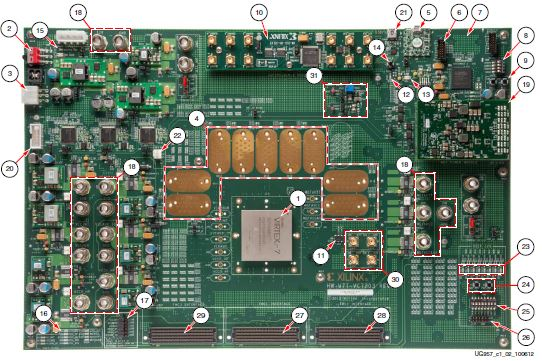
\includegraphics[width=0.86\textwidth]{FPGA}
		\caption{Vista Geral da FPGA VC7203 Virtex-7 retirada de \cite{R008}}
		\label{fig:fpgaVistaGeral}
	\end{center}
\end{figure}

A numeração 27, 28 e 29 correspondem aos conectores FMC disponíveis na FPGA a ser utilizada neste projeto. O número 27 corresponde ao conector JA2, 28 corresponde ao JA3 e 29 corresponde ao JA4. Estes conectores são usados como entradas e saídas de uma ligação, que neste caso em especifico será a uma placa HDMI, pois permitem uma ligação de alta velocidade (até 10 Gb/s). Estes três conectores HPC (High Pin Count) são compostos por 10x40 posições que permitem uma comunicação de alta velocidade por uma I/O cujo tamanho é relativamente pequeno. 

\textbf{O conector JA2 (FMC1 HPC) permite a seguinte conectividade:}
\begin{itemize}
	\item 68 pares que podem ser definidos pelo utilizador:
	\begin{itemize}
		\item 34 pares LA
		\item 17 pares HA
		\item 17 pares HB
	\end{itemize}
	\item 4 sinais de relógio diferenciais
\end{itemize}
\textbf{O conector JA3 (FMC2 HPC) permite a seguinte conectividade:}
\begin{itemize}
	\item 68 pares que podem ser definidos pelo utilizador:
	\begin{itemize}
		\item 34 pares LA
		\item 17 pares HA
		\item 17 pares HB
	\end{itemize}
	\item 4 sinais de relógio diferenciais
\end{itemize}
\textbf{O conector JA2 (FMC1 HPC) permite a seguinte conectividade:}
\begin{itemize}
	\item 65 pares que podem ser definidos pelo utilizador:
	\begin{itemize}
		\item 34 pares LA
		\item 16 pares HA
		\item 15 pares HB
	\end{itemize}
	\item 4 sinais de relógio diferenciais
\end{itemize}

Estes serão os conectores a ser utilizados e mais à frente neste relatório será explicado como é que os sinais são transmitidos. 

\subsection{Transmissor e Recetor} \label{batik}
Este \textit{hardware}, TB-FMCH-HDMI2, está dividido em 2 placas: o recetor (RX) que recebe o sinal recebido pelo cabo HDMI, faz a descodificação e envia o sinal para a FPGA, e o transmissor (TX) que faz o processo inverso, isto é, recebe o sinal proveniente da FPGA e transmite-o para o cabo HDMI para que possa chegar ao dispositivo de destino. 
\subsubsection{Recetor}\label{batik}
Na figura~\ref{fig:HDMIblocosRX} na página~\pageref{fig:HDMIblocosRX} é possível visualizar o diagrama de blocos do recetor disponível.
\begin{figure}[h!]
	\begin{center}
		\leavevmode
		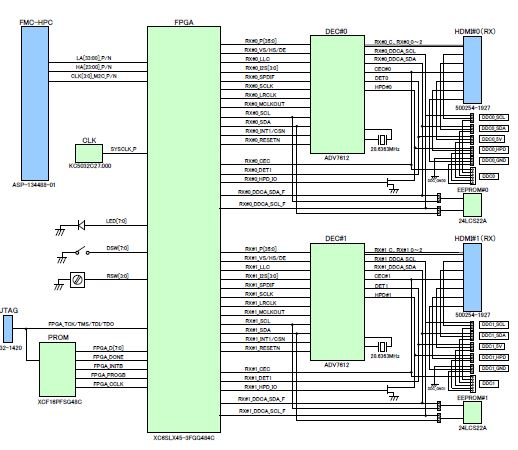
\includegraphics[width=0.7\textwidth]{HDMIrx}
		\caption{Diagrama de blocos de TB-FMCH-HDMI2 RX retirado de \cite{R009}}
		\label{fig:HDMIblocosRX}
	\end{center}
\end{figure}
As suas principais funções dividem-se nas seguintes:
\begin{enumerate}
	\item \textbf{Receção do Sinal HDMI (ADV7612 para a FPGA localizada na placa)}
	
	A receção do sinal HDMI é feita por um conector HDMI e usa um circuito integrado ADV7612BSWZ-P que recebe sinal HDMI e retira do mesmo os sinais a serem passados para a FPGA localizada na placa HDMI. O recetor tem também uma memória EEPROM (electrically erasable programmable read-only memory) que é usada para guardar dados EDID.
	\item \textbf{Interface com o conector FMC (da FPGA localizada na placa para o conector FMC)}
	
	Após passarem pela FPGA embebida (configura por \textit{default}) na placa são passados os seguintes sinais presentes na tabela 1:
\begin{table}[h!]
	\centering
	\begin{tabular}{|c|c|c|c|l}
		\hline
		\textbf{Nome do pin} & \textit{\textbf{Input/0utput}} & \textbf{FPGA para FMC} & \textbf{RX para a FPGA}        & \textbf{} \\ \hline
		CLK0\_M2C\_P         & \textit{Output}                & RX\#0\_LLC             & RX\#0 sinal LLC                &           \\ \cline{1-4}
		CLK1\_M2C\_P         & \textit{Output}                & RX\#1\_LLC             & RX\#1 sinal LLC                &           \\ \cline{1-4}
		LA00\_P\_CC          & \textit{Output}                & RX\#0\_VSYNC           & RX\#0\_VSYNC                   &           \\ \cline{1-4}
		LA01\_P\_CC          & \textit{Output}                & RX\#0\_HSYNC           & RX\#0\_HSYNC                   &           \\ \cline{1-4}
		LA02\_P              & \textit{Output}                & RX\#0\_DE              & RX\#0 data enable              &           \\ \cline{1-4}
		LA03\_P a LA32\_P    & \textit{Output}                & RX\#0\_P0 a RX\#0\_P29 & RX\#0 dados de vídeo de 0 a 29 &           \\ \cline{1-4}
		Nome do pin          & \textit{Input/0utput}          & FPGA para FMC          & RX para a FPGA                 &           \\ \cline{1-4}
		LA33\_P              & \textit{Input/Output}          & Não usado              & ----------                     &           \\ \cline{1-4}
		CLK0\_M2C\_N         & \textit{Input/Output}          & Não usado              & ----------                     &           \\ \cline{1-4}
		CLK1\_M2C\_N         & \textit{Input/Output}          & Não usado              & ----------                     &           \\ \hline
		LA00\_N\_CC          & \textit{Output}                & RX\#1\_VSYNC           & RX\#1\_VSYNC                   &           \\ \cline{1-4}
		LA01\_N\_CC          & \textit{Output}                & RX\#1\_HSYNC           & RX\#1\_HSYNC                   &           \\ \cline{1-4}
		LA02\_N              & \textit{Output}                & RX\#1\_DE              & RX\#1 data enable              &           \\ \cline{1-4}
		LA03\_N a LA32\_N    & \textit{Output}                & RX\#1\_P0 a RX\#1\_P29 & RX\#1 dados de vídeo de 0 a 29 &           \\ \cline{1-4}
		LA33\_P              & \textit{Input/Output}          & Não usado              & ----------                     &           \\ \cline{1-4}
		CLK2\_M2C\_P         & \textit{Input/Output}          & Não usado              & ----------                     &           \\ \cline{1-4}
		CLK3\_M2C\_P         & \textit{Input/Output}          & Não usado              & ----------                     &           \\ \cline{1-4}
		HA00\_P a HA23\_P    & \textit{Input/Output}          & Não usado              & ----------                     &           \\ \cline{1-4}
		CLK2\_M2C\_N         & \textit{Input/Output}          & Não usado              & ----------                     &           \\ \cline{1-4}
		CLK3\_M2C\_N         & \textit{Input/Output}          & Não usado              & ----------                     &           \\ \cline{1-4}
		HA00\_N a HA23\_N    & Input/Output                   & Não usado              & ----------                     &           \\ \cline{1-4}
	\end{tabular}
	\caption{HDMIdataRX}
	\label{Nomes dos pins da interface FMC de TB-FMCH-HDMI2 RX, adaptada de \cite{R009}}
\end{table}


\end{enumerate}


\subsubsection{Transmissor}\label{batik} 
\begin{figure}[h!]
	\begin{center}
		\leavevmode
		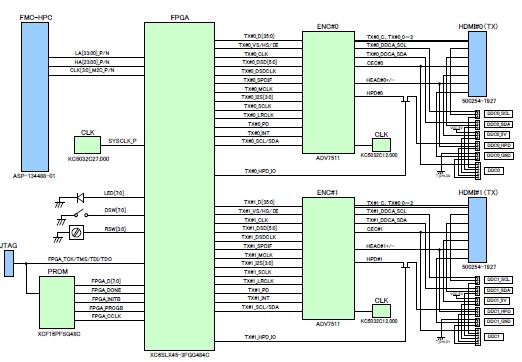
\includegraphics[width=0.7\textwidth]{HDMItx}
		\caption{Diagrama de blocos de TB-FMCH-HDMI2 TX retirado de \cite{R009}}
		\label{fig:HDMIblocosTX}
	\end{center}
\end{figure}
\chapter{HDMI}\label{chap:chap3}

Neste capítulo será abordado a primeira parte do trabalho proposto nesta dissertação que consiste em extraír os dados de imagem disponiveis numa ligação HDMI.

\section{\textit{Hardware} utilizado}

Tal como mencionado no sub-capítulo \ref{sec:HDMIinFPGA}, para efetuar a seleção dos dados é utlizado a placa TB-FMCH-HDMI que através das suas entradas e saída FMC de alta velocidade consegue enviar para a FPGA os sinais de imagem e som. 

Nas imagens \ref{fig:rx} e \ref{fig:tx} é possivel visualizar o recetor (TB-FMCH-HDMI2 RX) e o transmissor (TB-FMCH-HDMI2 TX) HDMI utilizados neste projeto. Em conjunto, estas duas placas são designadas apenas por TB-FMCH-HDMI2. Estas mesmas placas são constituidas por conectores HDMI, de seguida o sinal é enviado para um recetor ou transmissor HDMI, ADV7612 no caso do recetor e ADV7511 no caso do transmissor. Finalmente os sinais provenientes do recetor/transmissor são enviados para uma FGPA embebida na placa (XC6SLX45-3FGG484C) que, consoante a sua configuração, envia pelos conectores FMC os sinais de audio e video.

\subsection{Configurações da FPGA} \label{subsec:HDMIconfig}

A FPGA \textit{Spartan-6} (XC6SLX45-3FGG484C) embebida nas placas tem 3 configurações possiveis disponiveis. Estas configurações variam não só no suporte que têm que pode ser apenas imagem mas também imagem e audio, mas também no número de bits por imagem que as imagens a ser transmitidas podem ter. Estas diferenças passam a ser brevemente descritas nas próximas secções.

\subsubsection{Configuração por \textit{default}} \label{subsubsec:HDMIconfigdefault}

Esta configuração vem previamente configurada de fábrica nas placas e acaba por ser a mais simples de todas. Os dados enviados pelos conectores FMC são apenas referentes aos dados de imagem. As tabela \ref{table:HDMIdataRX} e \ref{table:HDMIdataTX} nas páginas \pageref{table:HDMIdataRX} e \pageref{table:HDMIdataTX} respectivamente identificam os pinos aos quais são atribuídas os sinais de dados de imagem HDMI tanto no recetor como no transmissor.

Esta configuração apenas transmite imagens RGB (\textit{Red Green Blue}) com 10 bits. Assim sendo, independetemente da formatação das imagens da fonte HDMI, apenas são transmitidos imagens em formato RGB. A tabela \ref{table:HDMIdataDefaultdetail} apresentada na página \pageref{table:HDMIdataDefaultdetail} mostra com  mais detalhe as portas utilizadas e ainda qual os bits que representam em cada imagem. 


\begin{table}[h!]
	\centering
	\begin{tabular}{|c|c|c|c|}
		\hline
		\textbf{PIN} & \textbf{FPGA -\textgreater FMC (RX)} & \textbf{FMC->FPGA (TX)} & \textbf{Descrição}       \\ \hline
		CLK0\_M2C\_P & RX\#O\_LLC                           & TX\#O\_DCLK                        & \textit{clock} dos pixeis         \\ \hline
		LA00\_P\_CC  & RX\#0\_VSYNC                         & TX\#0\_VSYNC                       & sincr. Vertical          \\ \hline
		LA01\_P\_CC  & RX\#0\_HSYNC                         & TX\#0\_HSYNC                       & sincr. Horizontal        \\ \hline
		LA02\_P      & RX\#0\_DE                            & TX\#0\_DE                          & sinal de dados ativos    \\ \hline
		LA03\_P      & RX\#0\_P0                            & TX\#0\_D0                          & Pixel de imagem B{[}0{]} \\ \hline
		LA04\_P      & RX\#0\_P1                            & TX\#0\_D1                          & Pixel de imagem B{[}1{]} \\ \hline
		LA05\_P      & RX\#0\_P2                            & TX\#0\_D2                          & Pixel de imagem B{[}2{]} \\ \hline
		LA06\_P      & RX\#0\_P3                            & TX\#0\_D3                          & Pixel de imagem B{[}3{]} \\ \hline
		LA07\_P      & RX\#0\_P4                            & TX\#0\_D4                          & Pixel de imagem B{[}4{]} \\ \hline
		LA08\_P      & RX\#0\_P5                            & TX\#0\_D5                          & Pixel de imagem B{[}5{]} \\ \hline
		LA09\_P      & RX\#0\_P6                            & TX\#0\_D6                          & Pixel de imagem B{[}6{]} \\ \hline
		LA10\_P      & RX\#0\_P7                            & TX\#0\_D7                          & Pixel de imagem B{[}7{]} \\ \hline
		LA11\_P      & RX\#0\_P8                            & TX\#0\_D8                          & Pixel de imagem B{[}8{]} \\ \hline
		LA12\_P      & RX\#0\_P9                            & TX\#0\_D9                          & Pixel de imagem B{[}9{]} \\ \hline
		LA13\_P      & RX\#0\_P10                           & TX\#0\_D10                         & Pixel de imagem G{[}0{]} \\ \hline
		LA14\_P      & RX\#0\_P11                           & TX\#0\_D11                         & Pixel de imagem G{[}1{]} \\ \hline
		LA15\_P      & RX\#0\_P12                           & TX\#0\_D12                         & Pixel de imagem G{[}2{]} \\ \hline
		LA16\_P      & RX\#0\_P13                           & TX\#0\_D13                         & Pixel de imagem G{[}3{]} \\ \hline
		LA17\_P\_CC  & RX\#0\_P14                           & TX\#0\_D14                         & Pixel de imagem G{[}4{]} \\ \hline
		LA18\_P\_CC  & RX\#0\_P15                           & TX\#0\_D15                         & Pixel de imagem G{[}5{]} \\ \hline
		LA19\_P      & RX\#0\_P16                           & TX\#0\_D16                         & Pixel de imagem G{[}6{]} \\ \hline
		LA20\_P      & RX\#0\_P17                           & TX\#0\_D17                         & Pixel de imagem G{[}7{]} \\ \hline
		LA21\_P      & RX\#0\_P18                           & TX\#0\_D18                         & Pixel de imagem G{[}8{]} \\ \hline
		LA22\_P      & RX\#0\_P19                           & TX\#0\_D19                         & Pixel de imagem G{[}9{]} \\ \hline
		LA23\_P      & RX\#0\_P20                           & TX\#0\_D20                         & Pixel de imagem R{[}0{]} \\ \hline
		LA24\_P      & RX\#0\_P21                           & TX\#0\_D21                         & Pixel de imagem R{[}1{]} \\ \hline
		LA25\_P      & RX\#0\_P22                           & TX\#0\_D22                         & Pixel de imagem R{[}2{]} \\ \hline
		LA26\_P      & RX\#0\_P23                           & TX\#0\_D23                         & Pixel de imagem R{[}3{]} \\ \hline
		LA27\_P      & RX\#0\_P24                           & TX\#0\_D24                         & Pixel de imagem R{[}4{]} \\ \hline
		LA28\_P      & RX\#0\_P25                           & TX\#0\_D25                         & Pixel de imagem R{[}5{]} \\ \hline
		LA29\_P      & RX\#0\_P26                           & TX\#0\_D26                         & Pixel de imagem R{[}6{]} \\ \hline
		LA30\_P      & RX\#0\_P27                           & TX\#0\_D27                         & Pixel de imagem R{[}7{]} \\ \hline
		LA31\_P      & RX\#0\_P28                           & TX\#0\_D28                         & Pixel de imagem R{[}8{]} \\ \hline
		LA32\_P      & RX\#0\_P29                           & TX\#0\_D29                         & Pixel de imagem R{[}9{]} \\ \hline
	\end{tabular}
	\caption{Localização dos pinos de dados utilizados em TB-FMCH-HDMI2 configurado por \textit{default}}
	\label{table:HDMIdataDefaultdetail}
\end{table}

É de notar ainda que esta configuração é capaz de suportar até dois canais (RX0 e TX0, RX1 e TX1), no entanto nesta tabela \ref{table:HDMIdataDefaultdetail} apenas são apresentados os dados correspondentes ao canal 0 pois apenas será necessário utilizar um canal neste projeto. 

\subsubsection{1 canal e suporte de audio} \label {subsubsec:HDMIconfig+audio}

Esta configuração trata-se de uma configuração capaz de suportar não só imagens em formato YCbCr mas também RGB com 12 bits, como também suporta audio em formato $I^{2}$S. A configuração da imagem está dependente da fonte HDMI, e é transmitida pelas placas tal como é emitida pela fonte, por outras palavras, se a fonte HDMI transmitir uma imagem em formato RGB, é nesse formato que chega ao destino, no entanto se for transmitida uma imagem no formato YCbCr é nesse formato que chega ao seu destino.



\subsubsection{2 canais melhorado} \label{subsubsec:HDMIconfigMelhorado}

\subsection{Configuração dos \textit{switches}}

\subsection{Arquiteturas Desenvolvidas}

\subsubsection{Transmissão de uma imagem gerada na FPGA}

\subsubsection{Transmissão de imagem entre dispositivos HDMI}

\subsubsection{Transmissão de imagem e som entre dispositivos HDMI}
\chapter{Transmissão dos dados em série}\label{chap:chap4}


\chapter{Conclusões e Trabalho Futuro} \label{chap:concl}

Adicionar as siglas:

PROM - Programmable read-only memory
SPDIF 

%% Comment next 2 commands if numbered appendices are not used
\appendix
\chapter{Descrição das portas das placas HDMI} \label{ap1:HDMI}

Este anexo aborda detalhadamente as conexões que as placas HDMI têm disponíveis para conexão com a FPGA consoante a configuração das mesmas. São apresentados todos os pinos que transmitem dados, qual o nome da ligação desses pinos nas placas HDMI e ainda a descrição dos sinais.
\section{Configuração por omissão} \label{ap1:default}

Esta secção apresenta todas as portas das placas HDMI configuradas por omissão (tanto recetora como transmissora) que transmitem dados que são utilizados no projeto na tabela \ref{table:HDMIdataDefaultdetail}. De referir que esta configuração suporta dois canais (0 e 1), no entanto apenas são apresentadas as portas relativas ao canal 0 pois é o único utilizado no projeto.

%\begin{longtable}[h!]
%	{@{}llll@{}}
%		\caption[Localização dos pinos de dados utilizados em nas placas HDMI configuradas por omissão]{Localização dos pinos de dados utilizados em nas placas HDMI configuradas por omissão, adaptada de \cite{R009}}
%		\label{table:HDMIdataDefaultdetail}
%		\hline
%		\centering	
%		\multicolumn{1}{c}{\textbf{PORTA}} & \multicolumn{1}{c}{\textbf{FPGA -\textgreater FMC (RX)}} & \multicolumn{1}{c}{\textbf{FMC -\textgreater FPGA (TX)}} & \multicolumn{1}{c}{\textbf{Descrição}} \\ \hline \endhead
%		CLK0\_M2C\_P & RX\#0\_LLC                           & TX\#0\_DCLK                        & Sinal de relógio dos pixeis         \\ 
%		LA00\_P\_CC  & RX\#0\_VSYNC                         & TX\#0\_VSYNC                       & Sincronização Vertical          \\ 
%		LA01\_P\_CC  & RX\#0\_HSYNC                         & TX\#0\_HSYNC                       & Sincronização Horizontal        \\ 
%		LA02\_P      & RX\#0\_DE                            & TX\#0\_DE                          & Sinal de dados ativos    \\ 
%		LA03\_P      & RX\#0\_P0                            & TX\#0\_D0                          & Pixel de imagem B{[}0{]} \\ 
%		LA04\_P      & RX\#0\_P1                            & TX\#0\_D1                          & Pixel de imagem B{[}1{]} \\ 
%		LA05\_P      & RX\#0\_P2                            & TX\#0\_D2                          & Pixel de imagem B{[}2{]} \\ 
%		LA06\_P      & RX\#0\_P3                            & TX\#0\_D3                          & Pixel de imagem B{[}3{]} \\ 
%		LA07\_P      & RX\#0\_P4                            & TX\#0\_D4                          & Pixel de imagem B{[}4{]} \\ 
%		LA08\_P      & RX\#0\_P5                            & TX\#0\_D5                          & Pixel de imagem B{[}5{]} \\ 
%		LA09\_P      & RX\#0\_P6                            & TX\#0\_D6                          & Pixel de imagem B{[}6{]} \\ 
%		LA10\_P      & RX\#0\_P7                            & TX\#0\_D7                          & Pixel de imagem B{[}7{]} \\ 
%		LA11\_P      & RX\#0\_P8                            & TX\#0\_D8                          & Pixel de imagem B{[}8{]} \\ 
%		LA12\_P      & RX\#0\_P9                            & TX\#0\_D9                          & Pixel de imagem B{[}9{]} \\ 
%		LA13\_P      & RX\#0\_P10                           & TX\#0\_D10                         & Pixel de imagem G{[}0{]} \\ 
%		LA14\_P      & RX\#0\_P11                           & TX\#0\_D11                         & Pixel de imagem G{[}1{]} \\ 
%		LA15\_P      & RX\#0\_P12                           & TX\#0\_D12                         & Pixel de imagem G{[}2{]} \\ 
%		LA16\_P      & RX\#0\_P13                           & TX\#0\_D13                         & Pixel de imagem G{[}3{]} \\ 
%		LA17\_P\_CC  & RX\#0\_P14                           & TX\#0\_D14                         & Pixel de imagem G{[}4{]} \\ 
%		LA18\_P\_CC  & RX\#0\_P15                           & TX\#0\_D15                         & Pixel de imagem G{[}5{]} \\ 
%		LA19\_P      & RX\#0\_P16                           & TX\#0\_D16                         & Pixel de imagem G{[}6{]} \\ 
%		LA20\_P      & RX\#0\_P17                           & TX\#0\_D17                         & Pixel de imagem G{[}7{]} \\ 
%		LA21\_P      & RX\#0\_P18                           & TX\#0\_D18                         & Pixel de imagem G{[}8{]} \\ 
%		LA22\_P      & RX\#0\_P19                           & TX\#0\_D19                         & Pixel de imagem G{[}9{]} \\ 
%		LA23\_P      & RX\#0\_P20                           & TX\#0\_D20                         & Pixel de imagem R{[}0{]} \\ 
%		LA24\_P      & RX\#0\_P21                           & TX\#0\_D21                         & Pixel de imagem R{[}1{]} \\ 
%		LA25\_P      & RX\#0\_P22                           & TX\#0\_D22                         & Pixel de imagem R{[}2{]} \\ 
%		LA26\_P      & RX\#0\_P23                           & TX\#0\_D23                         & Pixel de imagem R{[}3{]} \\ 
%		LA27\_P      & RX\#0\_P24                           & TX\#0\_D24                         & Pixel de imagem R{[}4{]} \\ 
%		LA28\_P      & RX\#0\_P25                           & TX\#0\_D25                         & Pixel de imagem R{[}5{]} \\ 
%		LA29\_P      & RX\#0\_P26                           & TX\#0\_D26                         & Pixel de imagem R{[}6{]} \\ 
%		LA30\_P      & RX\#0\_P27                           & TX\#0\_D27                         & Pixel de imagem R{[}7{]} \\ 
%		LA31\_P      & RX\#0\_P28                           & TX\#0\_D28                         & Pixel de imagem R{[}8{]} \\ 
%		LA32\_P      & RX\#0\_P29                           & TX\#0\_D29                         & Pixel de imagem R{[}9{]} \\ \hline
%
%\end{longtable}

\section{Suporte de um canal de imagem e áudio} \label {ap1:HDMIconfig+áudio}

Nesta secção são apresentadas todas as portas das placas HDMI configuradas para terem suporte de imagem e áudio num canal que enviam dados para a FPGA utilizados no projeto na tabela \ref{table:HDMI1canal+audioDETAIL}. São apresentados os nomes das portas nas placas, os nomes dos sinais tanto do lado do recetor como do transmissor e a sua descrição.

%\begin{longtable}[]
%	{@{}llll@{}}
%	\caption[Localização dos pinos de dados utilizados nas placas HDMI com a configuração de um canal e suporte de audio]{Localização dos pinos de dados utilizados nas placas HDMI com a configuração de um canal e suporte de audio, adaptada de \cite{R014}}
%	\label{table:HDMI1canal+audioDETAIL}
%	\hline
%	\centering
%		\multicolumn{1}{c}{\textbf{PORTA}} & \multicolumn{1}{c}{\textbf{FPGA -\textgreater FMC (RX)}} & \multicolumn{1}{c}{\textbf{FMC -\textgreater FPGA (TX)}} & \multicolumn{1}{c}{\textbf{Descrição}} \\ \hline \endhead		
%		CLK0\_M2C\_P & RX\#0\_LLC                         & TX\#0\_DCLK                          & Sinal de relógio dos pixeis          \\ 
%		LA00\_P\_CC  & RX\#0\_VSYNC                       & TX\#0\_VSYNC                         & Sincronização vertical               \\ 
%		LA01\_P\_CC  & RX\#0\_HSYNC                       & TX\#0\_HSYNC                         & Sincronização horizontal             \\ 
%		LA02\_P      & RX\#0\_DE                          & TX\#0\_DE                            & Sinal de dados ativos                \\ 
%		LA03\_P      & RX\#0\_P0                          & TX\#0\_D0                            & Pixel de Imagem Cb{[}0{]}/B{[}0{]}   \\ 
%		LA04\_P      & RX\#0\_P1                          & TX\#0\_D1                            & Pixel de Imagem Cb{[}1{]}/B{[}1{]}   \\ 
%		LA05\_P      & RX\#0\_P2                          & TX\#0\_D2                            & Pixel de Imagem Cb{[}2{]}/B{[}2{]}   \\ 
%		LA06\_P      & RX\#0\_P3                          & TX\#0\_D3                            & Pixel de Imagem Cb{[}3{]}/B{[}3{]}   \\ 
%		LA07\_P      & RX\#0\_P4                          & TX\#0\_D4                            & Pixel de Imagem Cb{[}4{]}/B{[}4{]}   \\ 
%		LA08\_P      & RX\#0\_P5                          & TX\#0\_D5                            & Pixel de Imagem Cb{[}5{]}/B{[}5{]}   \\ 
%		LA09\_P      & RX\#0\_P6                          & TX\#0\_D6                            & Pixel de Imagem Cb{[}6{]}/B{[}6{]}   \\ 
%		LA10\_P      & RX\#0\_P7                          & TX\#0\_D7                            & Pixel de Imagem Cb{[}7{]}/B{[}7{]}   \\ 
%		LA11\_P      & RX\#0\_P8                          & TX\#0\_D8                            & Pixel de Imagem Cb{[}8{]}/B{[}8{]}   \\ 
%		LA12\_P      & RX\#0\_P9                          & TX\#0\_D9                            & Pixel de Imagem Cb{[}9{]}/B{[}9{]}   \\ 
%		LA13\_P      & RX\#0\_P10                         & TX\#0\_D10                           & Pixel de Imagem Cb{[}10{]}/B{[}10{]} \\ 
%		LA14\_P      & RX\#0\_P11                         & TX\#0\_D11                           & Pixel de Imagem Cb{[}11{]}/B{[}11{]} \\ 
%		LA15\_P      & RX\#0\_P12                         & TX\#0\_D12                           & Pixel de Imagem Y{[}0{]}/G{[}0{]}    \\ 
%		LA16\_P      & RX\#0\_P13                         & TX\#0\_D13                           & Pixel de Imagem Y{[}1{]}/G{[}1{]}    \\ 
%		LA17\_P\_CC  & RX\#0\_P14                         & TX\#0\_D14                           & Pixel de Imagem Y{[}2{]}/G{[}2{]}    \\ 
%		LA18\_P\_CC  & RX\#0\_P15                         & TX\#0\_D15                           & Pixel de Imagem Y{[}3{]}/G{[}3{]}    \\ 
%		LA19\_P      & RX\#0\_P16                         & TX\#0\_D16                           & Pixel de Imagem Y{[}4{]}/G{[}4{]}    \\ 
%		LA20\_P      & RX\#0\_P17                         & TX\#0\_D17                           & Pixel de Imagem Y{[}5{]}/G{[}5{]}    \\ 
%		LA21\_P      & RX\#0\_P18                         & TX\#0\_D18                           & Pixel de Imagem Y{[}6{]}/G{[}6{]}    \\ 
%		LA22\_P      & RX\#0\_P19                         & TX\#0\_D19                           & Pixel de Imagem Y{[}7{]}/G{[}7{]}    \\ 
%		LA23\_P      & RX\#0\_P20                         & TX\#0\_D20                           & Pixel de Imagem Y{[}8{]}/G{[}8{]}    \\ 
%		LA24\_P      & RX\#0\_P21                         & TX\#0\_D21                           & Pixel de Imagem Y{[}9{]}/G{[}9{]}    \\ 
%		LA25\_P      & RX\#0\_P22                         & TX\#0\_D22                           & Pixel de Imagem Y{[}10{]}/G{[}10{]}  \\ 
%		LA26\_P      & RX\#0\_P23                         & TX\#0\_D23                           & Pixel de Imagem Y{[}11{]}/G{[}11{]}  \\ 
%		LA27\_P      & RX\#0\_P24                         & TX\#0\_D24                           & Pixel de Imagem Cr{[}0{]}/R{[}0{]}   \\ 
%		LA28\_P      & RX\#0\_P25                         & TX\#0\_D25                           & Pixel de Imagem Cr{[}1{]}/R{[}1{]}   \\ 
%		LA29\_P      & RX\#0\_P26                         & TX\#0\_D26                           & Pixel de Imagem Cr{[}2{]}/R{[}2{]}   \\ 
%		LA30\_P      & RX\#0\_P27                         & TX\#0\_D27                           & Pixel de Imagem Cr{[}3{]}/R{[}3{]}   \\ 
%		LA31\_P      & RX\#0\_P28                         & TX\#0\_D28                           & Pixel de Imagem Cr{[}4{]}/R{[}4{]}   \\ 
%		LA32\_P      & RX\#0\_P29                         & TX\#0\_D29                           & Pixel de Imagem Cr{[}5{]}/R{[}5{]}   \\ 
%		LA00\_N\_CC & \begin{tabular}[l]{@{}l@{}}RX\#0\_Input \\ video status{[}0{]}\end{tabular}   & \begin{tabular}[l]{@{}l@{}}TX\#0\_Input \\ video status{[}0{]}\end{tabular} & Formato do video (2D/3D) 			   \\ 
%	
%		LA01\_N\_CC & \begin{tabular}[l]{@{}l@{}}RX\#0\_Input \\ video status{[}1{]}\end{tabular}    & \begin{tabular}[l]{@{}l@{}}TX\#0\_Input \\ video status{[}1{]}\end{tabular}       & Formato do video (2D/3D)   \\ 
%		LA19\_N      & RX\#0\_MCLK                        & TX\#0\_MCLK                          & \textit{Master Clock} de som     \\ 
%		LA20\_N      & RX\#0\_SCLK                        & TX\#0\_SCLK                          & \textit{Serial Clock} de som     \\ 
%		LA21\_N      & RX\#0\_AP0                         & TX\#0\_AP0                           & Dados de Som SPDIF                   \\ 
%		LA22\_N      & RX\#0\_AP1                         & TX\#0\_AP1                           & Dados de Som I2S {[}0{]}             \\ 
%		LA23\_N      & RX\#0\_AP2                         & TX\#0\_AP2                           & Dados de Som I2S {[}1{]}             \\ 
%		LA24\_N      & RX\#0\_AP3                         & TX\#0\_AP3                           & Dados de Som I2S {[}2{]}             \\ 
%		LA25\_N      & RX\#0\_AP4                         & TX\#0\_AP4                           & Dados de Som I2S {[}3{]}             \\ 
%		LA26\_N      & RX\#0\_AP5                         & TX\#0\_AP5                           & Sinal de relógio LR (left/right)     \\ 
%		LA27\_N      & RX\#0\_P30                         & TX\#0\_D30                           & Pixel de Imagem Cr{[}6{]}/R{[}6{]}   \\ 
%		LA28\_N      & RX\#0\_P31                         & TX\#0\_D31                           & Pixel de Imagem Cr{[}7{]}/R{[}7{]}   \\ 
%		LA29\_N      & RX\#0\_P32                         & TX\#0\_D32                           & Pixel de Imagem Cr{[}8{]}/R{[}8{]}   \\ 
%		LA30\_N      & RX\#0\_P33                         & TX\#0\_D33                           & Pixel de Imagem Cr{[}9{]}/R{[}9{]}   \\ 
%		LA31\_N      & RX\#0\_P34                         & TX\#0\_D34                           & Pixel de Imagem Cr{[}10{]}/R{[}10{]} \\ 
%		LA32\_N      & RX\#0\_P35                         & TX\#0\_D35                           & Pixel de Imagem Cr{[}11{]}/R{[}11{]} \\ \hline
%\end{longtable}

\section{Suporte de dois canais de imagem melhorado} \label{ap1:HDMIconfigMelhorado}

Nesta secção são apresentados os dados enviados pelas placas HDMI configuradas para a versão de suporte de imagem em dois canais melhorada. Para cada porta são apresentados os nomes dos sinais tanto na placa transmissora como recetora e também é descrito o seu funcionamento. De notar que esta configuração suporta dois canais, mas na tabela \ref{table:HDMI1canal_melhorado} apenas é apresentado o canal 0, visto que o canal 1 não é utilizado.
\\


%\begin{longtable}[h!]
%	{@{}llll@{}}
%	\caption[Localização dos pinos de dados utilizados nas placas HDMI com a configuração de suporte de dois canais melhorado]{Localização dos pinos de dados utilizados nas placas HDMI com a configuração de suporte de dois canais melhorado, adaptada de \cite{R013}}
%	\label{table:HDMI1canal_melhorado}
%	\hline
%	\centering
%	\multicolumn{1}{c}{\textbf{PORTA}} & \multicolumn{1}{c}{\textbf{FPGA -\textgreater FMC (RX)}} & \multicolumn{1}{c}{\textbf{FMC -\textgreater FPGA (TX)}} & \multicolumn{1}{c}{\textbf{Descrição}} \\ \hline \endhead
%	CLK0\_M2C\_P & RX\#0\_LLC          				& TX\#0\_DCLK                          & Sinal de relógio dos pixeis 			\\ 
%	%CLK1\_M2C\_N & RX\#1\_LLC           			 & TX\#1\_DCLK                          & Sinal de relógio dos pixeis 			\\ \hline
%	LA00\_P\_CC  & RX\#0\_VSYNC         			  & TX\#0\_VSYNC                         & Sincronização vertical         		\\ 
%	LA01\_P\_CC  & RX\#0\_HSYNC         		  & TX\#0\_HSYNC                         & Sincronização horizontal       		\\ 
%	LA02\_P      & RX\#0\_DE            				   & TX\#0\_DE                            & Sinal de dados ativos          		\\
%	LA03\_P      & RX\#0\_P0            				   & TX\#0\_D0                            & Pixel de Imagem Cb{[}0{]}/B{[}0{]}   \\
%	LA04\_P      & RX\#0\_P1            		      & TX\#0\_D1                            & Pixel de Imagem Cb{[}1{]}/B{[}1{]}   \\ 
%	LA05\_P      & RX\#0\_P2            			      & TX\#0\_D2                            & Pixel de Imagem Cb{[}2{]}/B{[}2{]}   \\ 
%	LA06\_P      & RX\#0\_P3            			      & TX\#0\_D3                            & Pixel de Imagem Cb{[}3{]}/B{[}3{]}   \\ 
%	LA07\_P      & RX\#0\_P4            			      & TX\#0\_D4                            & Pixel de Imagem Cb{[}4{]}/B{[}4{]}   \\ 
%	LA08\_P      & RX\#0\_P5            			      & TX\#0\_D5                            & Pixel de Imagem Cb{[}5{]}/B{[}5{]}   \\ 
%	LA09\_P      & RX\#0\_P6            		     & TX\#0\_D6                            & Pixel de Imagem Cb{[}6{]}/B{[}6{]}   \\ 
%	LA10\_P      & RX\#0\_P7            			     & TX\#0\_D7                            & Pixel de Imagem Cb{[}7{]}/B{[}7{]}   \\
%	LA11\_P      & RX\#0\_P8            			     & TX\#0\_D8                            & Pixel de Imagem Cb{[}8{]}/B{[}8{]}   \\ 
%	LA12\_P      & RX\#0\_P9            		      & TX\#0\_D9                            & Pixel de Imagem Cb{[}9{]}/B{[}9{]}   \\
%	LA13\_P      & RX\#0\_P10           		      & TX\#0\_D10                           &Pixel de Imagem Y{[}0{]}/G{[}0{]} 	\\ 
%	LA14\_P      & RX\#0\_P11           		     & TX\#0\_D11                           & Pixel de Imagem Y{[}1{]}/G{[}1{]}	\\ 
%	LA15\_P      & RX\#0\_P12          				     & TX\#0\_D12                           & Pixel de Imagem Y{[}2{]}/G{[}2{]}    \\
%	LA16\_P      & RX\#0\_P13           			      & TX\#0\_D13                           & Pixel de Imagem Y{[}3{]}/G{[}3{]}    \\ 
%	LA17\_P\_CC  & RX\#0\_P14           		  & TX\#0\_D14                           & Pixel de Imagem Y{[}4{]}/G{[}4{]}    \\ 
%	LA18\_P\_CC  & RX\#0\_P15           		  & TX\#0\_D15                           & Pixel de Imagem Y{[}5{]}/G{[}5{]}    \\ 
%	LA19\_P      & RX\#0\_P16           			      & TX\#0\_D16                           & Pixel de Imagem Y{[}6{]}/G{[}6{]}   	\\ 
%	LA20\_P      & RX\#0\_P17           			      & TX\#0\_D17                           & Pixel de Imagem Y{[}7{]}/G{[}7{]}    \\ 
%	LA21\_P      & RX\#0\_P18           		      & TX\#0\_D18                           & Pixel de Imagem Y{[}8{]}/G{[}8{]}    \\ 
%	LA22\_P      & RX\#0\_P19           			     & TX\#0\_D19                           & Pixel de Imagem Y{[}9{]}/G{[}9{]}    \\
%	LA23\_P      & RX\#0\_P20           		      & TX\#0\_D20                           & Pixel de Imagem Cr{[}0{]}/R{[}0{]}    \\ 
%	LA24\_P      & RX\#0\_P21           		     & TX\#0\_D21                           & Pixel de Imagem Cr{[}1{]}/R{[}1{]}   \\ 
%	LA25\_P      & RX\#0\_P22           		      & TX\#0\_D22                           & Pixel de Imagem Cr{[}2{]}/R{[}2{]}  \\ 
%	LA26\_P      & RX\#0\_P23          			     & TX\#0\_D23                           & Pixel de Imagem Cr{[}3{]}/R{[}3{]}  \\ 
%	LA27\_P      & RX\#0\_P24           			      & TX\#0\_D24                           & Pixel de Imagem Cr{[}4{]}/R{[}4{]}  \\ 
%	LA28\_P      & RX\#0\_P25           		      & TX\#0\_D25                           & Pixel de Imagem Cr{[}5{]}/R{[}5{]}   \\
%	LA29\_P      & RX\#0\_P26           		      & TX\#0\_D26                           & Pixel de Imagem Cr{[}6{]}/R{[}6{]}   \\ 
%	LA30\_P      & RX\#0\_P27           		      & TX\#0\_D27                           & Pixel de Imagem Cr{[}7{]}/R{[}7{]}   \\ 
%	LA31\_P      & RX\#0\_P28           			      & TX\#0\_D28                           & Pixel de Imagem Cr{[}8{]}/R{[}8{]}   \\
%	LA32\_P      & RX\#0\_P29           		      & TX\#0\_D29                           & Pixel de Imagem Cr{[}9{]}/R{[}9{]}   	\\ 
%	
%	CLK0\_M2C\_N & \begin{tabular}[l]{@{}l@{}}RX\#0\_Input \\ video status{[}0{]}\end{tabular}   & \begin{tabular}[l]{@{}l@{}}TX\#0\_Input \\ video status{[}0{]}\end{tabular} & Formato do video (2D/3D) 			   \\ 
%		
%	CLK1\_M2C\_N & \begin{tabular}[l]{@{}l@{}}RX\#0\_Input \\ video status{[}1{]}\end{tabular}    & \begin{tabular}[l]{@{}l@{}}TX\#0\_Input \\ video status{[}1{]}\end{tabular}       & Formato do video (2D/3D)   \\ 
%%	LA33\_P      & \begin{tabular}[c]{@{}c@{}}RX\#1\_Input \\ video status{[}0{]}\end{tabular}    	   & \begin{tabular}[c]{@{}c@{}}TX\#1\_Input \\ video status{[}0{]}\end{tabular}       & Formato do video (2D/3D) 			   \\ \hline
%%	LA33\_N      & \begin{tabular}[c]{@{}c@{}}RX\#1\_Input \\ video status{[}1{]}\end{tabular}   	   & \begin{tabular}[c]{@{}c@{}}TX\#1\_Input \\ video status{[}1{]}\end{tabular}       & Formato do video (2D/3D) 			   \\ \hline
%%	LA00\_N\_CC  & RX\#1\_VSYNC                      & TX\#1\_VSYNC                         & Sincronização vertical         		\\ \hline
%%	LA01\_N\_CC  & RX\#1\_HSYNC                     & TX\#1\_HSYNC                         & Sincronização horizontal       		\\ \hline
%%	LA02\_N      & RX\#1\_DE                        & TX\#1\_DE                            & Sinal de dados ativos          		\\ \hline
%%	LA03\_N      & RX\#1\_P0                         & TX\#1\_D0                            & Pixel de Imagem B{[}0{]}   \\ \hline
%%	LA04\_N      & RX\#1\_P1                        & TX\#1\_D1                            & Pixel de Imagem B{[}1{]}   \\ \hline
%%	LA05\_N      & RX\#1\_P2                         & TX\#1\_D2                            & Pixel de Imagem B{[}2{]}   \\ \hline
%%	LA06\_N      & RX\#1\_P3                         & TX\#1\_D3                            & Pixel de Imagem B{[}3{]}   \\ \hline
%%	LA07\_N      & RX\#1\_P4                        & TX\#1\_D4                            & Pixel de Imagem B{[}4{]}   \\ \hline
%%	LA08\_N      & RX\#1\_P5                       & TX\#1\_D5                            & Pixel de Imagem B{[}5{]}   \\ \hline
%%	LA09\_N      & RX\#1\_P6                         & TX\#1\_D6                            & Pixel de Imagem B{[}6{]}   \\ \hline
%%	LA10\_N      & RX\#1\_P7                        & TX\#1\_D7                            & Pixel de Imagem B{[}7{]}   \\ \hline
%%	LA11\_N      & RX\#1\_P8                        & TX\#1\_D8                            & Pixel de Imagem B{[}8{]}   \\ \hline
%%	LA12\_N      & RX\#1\_P9                        & TX\#1\_D9                            & Pixel de Imagem B{[}9{]}   \\ \hline
%%	LA13\_N      & RX\#1\_P10                        & TX\#1\_D10                           & Pixel de Imagem G{[}0{]} 	\\ \hline
%%	LA14\_N      & RX\#1\_P11                        & TX\#1\_D11                           & Pixel de Imagem G{[}1{]}	\\ \hline
%%	LA15\_N      & RX\#1\_P12                      & TX\#1\_D12                           & Pixel de Imagem G{[}2{]}    \\ \hline
%%	LA16\_N      & RX\#1\_P13                      & TX\#1\_D13                           & Pixel de Imagem G{[}3{]}    \\ \hline
%%	LA17\_N\_CC  & RX\#1\_P14                        & TX\#1\_D14                           & Pixel de Imagem G{[}4{]}    \\ \hline
%%	LA18\_N\_CC  & RX\#1\_P15                        & TX\#1\_D15                           & Pixel de Imagem G{[}5{]}    \\ \hline
%%	LA19\_N      & RX\#1\_P16                        & TX\#1\_D16                           & Pixel de Imagem G{[}6{]}   	\\ \hline
%%	LA20\_N      & RX\#1\_P17                        & TX\#1\_D17                           & Pixel de Imagem G{[}7{]}    \\ \hline
%%	LA21\_N      & RX\#1\_P18                       & TX\#1\_D18                           & Pixel de Imagem G{[}8{]}    \\ \hline
%%	LA22\_N      & RX\#1\_P19                       & TX\#1\_D19                           & Pixel de Imagem G{[}9{]}    \\ \hline
%%	LA23\_N      & RX\#1\_P20                       & TX\#1\_D20                           & Pixel de Imagem R{[}0{]}    \\ \hline
%%	LA24\_N      & RX\#1\_P21                       & TX\#1\_D21                           & Pixel de Imagem R{[}1{]}   \\ \hline
%%	LA25\_N      & RX\#1\_P22                       & TX\#1\_D22                           & Pixel de Imagem R{[}2{]}  \\ \hline
%%	LA26\_N      & RX\#1\_P23                      & TX\#1\_D23                           & Pixel de Imagem R{[}3{]}  \\ \hline
%%	LA27\_N      & RX\#1\_P24                        & TX\#1\_D24                           & Pixel de Imagem R{[}4{]}  \\ \hline
%%	LA28\_N      & RX\#1\_P25                      & TX\#1\_D25                           & Pixel de Imagem R{[}5{]}   \\ \hline
%%	LA29\_N      & RX\#1\_P26                      & TX\#1\_D26                           & Pixel de Imagem R{[}6{]}   \\ \hline
%%	LA30\_N      & RX\#1\_P27                       & TX\#1\_D27                           & Pixel de Imagem R{[}7{]}   \\ \hline
%%	LA31\_N      & RX\#1\_P28                       & TX\#1\_D28                           & Pixel de Imagem R{[}8{]}   \\ \hline
%%	LA32\_N      & RX\#1\_P29                       & TX\#1\_D29                           & Pixel de Imagem R{[}9{]}   	\\ \hline
%	\hline
%\end{longtable}

%%----------------------------------------
%% Final materials
%%----------------------------------------

%% Bibliography
%% Comment the next command if BibTeX file not used, 
%% Assumes that bibliography is in ``myrefs.bib''
%%\PrintBib{myrefs}
\bibliographystyle{ieeetr}
\bibliography{myrefs}



%% Index
%% Uncomment next command if index is required, 
%% don't forget to run ``makeindex tese'' command
%\PrintIndex

\end{document}
